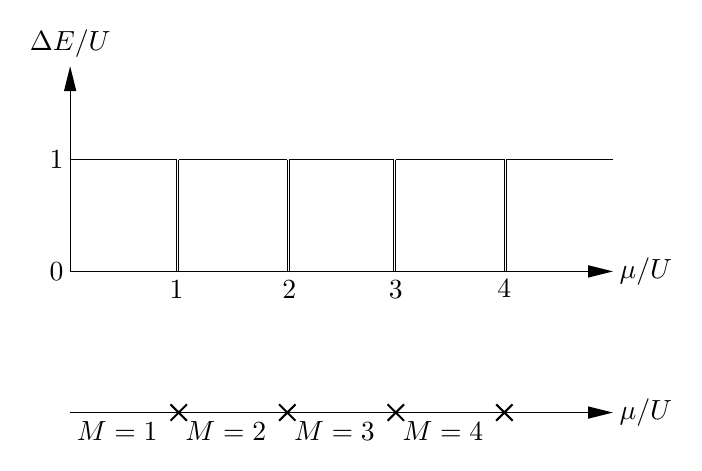
\begin{tikzpicture}[x=0.75pt,y=0.75pt,yscale=-1,xscale=1]
    %uncomment if require: \path (0,300); %set diagram left start at 0, and has height of 300
    
    %Straight Lines [id:da3506585102222235] 
    \draw    (100,155) -- (152.3,155) ;
    %Straight Lines [id:da895220782085971] 
    \draw    (152.3,155) -- (204.6,155) ;
    %Straight Lines [id:da8373948832562332] 
    \draw    (204.6,155) -- (256.9,155) ;
    %Straight Lines [id:da27683478112896753] 
    \draw    (256.9,155) -- (309.2,155) ;
    %Straight Lines [id:da32246801352481147] 
    \draw    (309.2,155) -- (359.5,155) ;
    \draw [shift={(361.5,155)}, rotate = 180] [fill={rgb, 255:red, 0; green, 0; blue, 0 }  ][line width=0.08]  [draw opacity=0] (12,-3) -- (0,0) -- (12,3) -- cycle    ;
    %Straight Lines [id:da4206170110777874] 
    \draw    (100,155) -- (100,58.17) ;
    \draw [shift={(100,56.17)}, rotate = 90] [fill={rgb, 255:red, 0; green, 0; blue, 0 }  ][line width=0.08]  [draw opacity=0] (12,-3) -- (0,0) -- (12,3) -- cycle    ;
    %Straight Lines [id:da8662027660822462] 
    \draw    (100,223) -- (152.3,223) ;
    \draw [shift={(152.3,223)}, rotate = 45] [color={rgb, 255:red, 0; green, 0; blue, 0 }  ][line width=0.75]    (-5.59,0) -- (5.59,0)(0,5.59) -- (0,-5.59)   ;
    %Straight Lines [id:da34431304247304895] 
    \draw    (152.3,223) -- (204.6,223) ;
    \draw [shift={(204.6,223)}, rotate = 45] [color={rgb, 255:red, 0; green, 0; blue, 0 }  ][line width=0.75]    (-5.59,0) -- (5.59,0)(0,5.59) -- (0,-5.59)   ;
    %Straight Lines [id:da12932606251036693] 
    \draw    (204.6,223) -- (256.9,223) ;
    \draw [shift={(256.9,223)}, rotate = 45] [color={rgb, 255:red, 0; green, 0; blue, 0 }  ][line width=0.75]    (-5.59,0) -- (5.59,0)(0,5.59) -- (0,-5.59)   ;
    %Straight Lines [id:da7717873736628669] 
    \draw    (256.9,223) -- (309.2,223) ;
    \draw [shift={(309.2,223)}, rotate = 45] [color={rgb, 255:red, 0; green, 0; blue, 0 }  ][line width=0.75]    (-5.59,0) -- (5.59,0)(0,5.59) -- (0,-5.59)   ;
    %Straight Lines [id:da2272617661619305] 
    \draw    (309.2,223) -- (359.5,223) ;
    \draw [shift={(361.5,223)}, rotate = 180] [fill={rgb, 255:red, 0; green, 0; blue, 0 }  ][line width=0.08]  [draw opacity=0] (12,-3) -- (0,0) -- (12,3) -- cycle    ;
    %Straight Lines [id:da251190008171309] 
    \draw    (152.3,101.17) -- (152.3,155) ;
    %Straight Lines [id:da13453595010909813] 
    \draw    (100,101) -- (151.3,101) ;
    %Straight Lines [id:da2967390574830482] 
    \draw    (152.3,101) -- (204.6,101) ;
    %Straight Lines [id:da14966038607228227] 
    \draw    (205.6,101) -- (255.9,101) ;
    %Straight Lines [id:da39911687911719484] 
    \draw    (256.9,101) -- (309.2,101) ;
    %Straight Lines [id:da8046998449068332] 
    \draw    (310.2,101) -- (361.5,101) ;
    %Straight Lines [id:da3273431043505528] 
    \draw    (204.6,101.17) -- (204.6,155) ;
    %Straight Lines [id:da5075124395721766] 
    \draw    (151.3,101.17) -- (151.3,155) ;
    %Straight Lines [id:da09048481100296502] 
    \draw    (205.6,101.17) -- (205.6,155) ;
    %Straight Lines [id:da35407753871379377] 
    \draw    (255.9,101.17) -- (255.9,155) ;
    %Straight Lines [id:da16596437824405674] 
    \draw    (309.2,101) -- (309.2,154.83) ;
    %Straight Lines [id:da6217231332099147] 
    \draw    (256.9,101.17) -- (256.9,155) ;
    %Straight Lines [id:da23474959772637116] 
    \draw    (310.2,101) -- (310.2,154.83) ;
    
    % Text Node
    \draw (363.5,155) node [anchor=west] [inner sep=0.75pt]    {$\mu /U$};
    % Text Node
    \draw (100,53.17) node [anchor=south] [inner sep=0.75pt]    {$\Delta E/U$};
    % Text Node
    \draw (363.5,223) node [anchor=west] [inner sep=0.75pt]    {$\mu /U$};
    % Text Node
    \draw (98,101) node [anchor=east] [inner sep=0.75pt]   [align=left] {1};
    % Text Node
    \draw (98,155) node [anchor=east] [inner sep=0.75pt]   [align=left] {0};
    % Text Node
    \draw (151.3,158) node [anchor=north] [inner sep=0.75pt]   [align=left] {1};
    % Text Node
    \draw (205.6,158) node [anchor=north] [inner sep=0.75pt]   [align=left] {2};
    % Text Node
    \draw (256.9,158) node [anchor=north] [inner sep=0.75pt]   [align=left] {3};
    % Text Node
    \draw (309.2,157.83) node [anchor=north] [inner sep=0.75pt]   [align=left] {4};
    % Text Node
    \draw (102,226) node [anchor=north west][inner sep=0.75pt]    {$M=1$};
    % Text Node
    \draw (154.3,226) node [anchor=north west][inner sep=0.75pt]    {$M=2$};
    % Text Node
    \draw (206.6,226) node [anchor=north west][inner sep=0.75pt]    {$M=3$};
    % Text Node
    \draw (258.9,226) node [anchor=north west][inner sep=0.75pt]    {$M=4$};
    
    
    \end{tikzpicture}
    